\chapter{Implementacija i korisničko sučelje}
		
		
		\section{Korištene tehnologije i alati}
		
			\text Komunikacija u timu realizirana je korištenjem aplikacija WhatsApp\footnote{\url{https://www.whatsapp.com/}} i Messenger za Facebook\footnote{\url{https://https://www.messenger.com/}}, a sastanci su održavani putem platformi Microsoft Teams\footnote{\url{https://www.microsoft.com/hr-hr/microsoft-365/microsoft-teams/}} te Discord\footnote{url{https://discord.com/}}. Za izradu UML dijagrama korišten je alat Astah UML\footnote{\url{https://astah.net/products/astah-uml/}}, a kao sustav za upravljanje izvornim kodom Git\footnote{\url{https://git-scm.com/}}. Udaljeni repozitorij projekta dostupan je na web platformi GitLab\footnote{\url{https://gitlab.com/}}.
			
			Kao razvojno okruženje korišten je Visual Studio Code\footnote{\url{https://code.visualstudio.com/}} – uređivač koda tvrtke Microsoft. Dostupan je za Window, Linux i macOS. Uključuje podršku za otklanjanje pogrešaka, isticanje sintakse, inteligentno dovršavanje koda, refaktoriranje koda i ugrađeni Git. Inicijalno ima ugrađenu podršku za JavaScript, TypeScript i Node.js, no ima bogat sustav ekstenzija za druge jezike (na primjer C++, Java, Phyton, Dart) i druge radne okvire (.NET, Unity…)
			
			Aplikacija je napisana korištenjem softera Flutter\footnote{\url{https://flutter.dev/}} i programskog jezika Dart\footnote{\url{https://dart.dev/}}. Flutter je softver za razvoj korisničkog sučelja otvorenog koda, razvijen od tvrtke Google. Omogućava višeplatformski razvoj korištenjem jednog koda te jedostavnost izrade aplikacija. Flutter koristi programski jezik Dart, kojim je realiziran i frontend i backend.
			
			Baza podataka nalazi se na poslužitelju u oblaku Firestore\footnote{\url{https://firebase.google.com/docs/firestore}}. 
			
			
			
			\eject 
		
	
		\section{Ispitivanje programskog rješenja}
			
			\subsection{Ispitivanje komponenti}
			
			Ispitivanje komponenti verificira rad programskih dijelova koje je moguće neovisno zasebno ispitati. Za ispitivanje smo koristili Flutter Test i MockFirebase priključke.
			
			Kod na slici \ref{fig:addCourse} provodi ispitivanje funkcionalnosti stvaranja tečaja korištenjem funkcije addCourse unutar razreda CoursesDB. U testu su obavljena tri dodavanja tečaja. Nakon toga se provjerava sadrži li kolekcija tri elementa.
			
			\begin{figure}[h]
				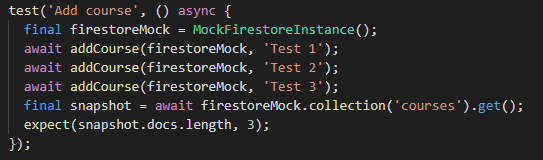
\includegraphics[scale=0.75]{slike/addCourse.PNG}
				\centering
				\caption{addCourse}
				\label{fig:addCourse}
			\end{figure}
			
			Slika \ref{fig:addUniqueUser} prikazuje kod koji provjerava ispravnost dodavanja novog korisnika u bazu podataka pomoću metode addUser. E-mail adrese su jedinstvene unutar baze podataka, odnosno nije dozvoljeno da dva korisnika imaju istu e-mail adresu. Prva dva e-maila su različita i nakon prva dva poziva funkcije addUser dokument bi trebao imati dva elementa. Treći poziv metode sadrži već korištenu e-mail adresu i zbog toga se očekuje da je veličina kolekcije i dalje dva.
			
			\begin{figure}[h]
				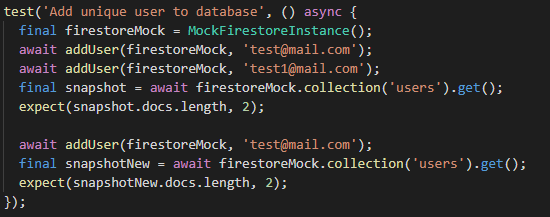
\includegraphics[scale=0.75]{slike/addUniqueUser.PNG}
				\centering
				\caption{Dodavanje novog korisnika}
				\label{fig:addUniqueUser}
			\end{figure}
			
			
			\eject
			
			Kod na slici \ref{fig:noUser} služi za provjeru prijavljenih korisnika. Test očekuje da nema prijavljenih korisnika, tj. da je user jednak null.
			
			\begin{figure}[h]
				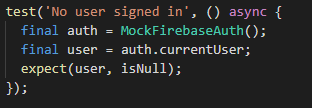
\includegraphics[scale=0.75]{slike/noUser.PNG}
				\centering
				\caption{Provjera prijavljenih korisnika}
				\label{fig:noUser}
			\end{figure}
			
			Prijava korisnika prikazana je na slici \ref{fig:login}. Nakon unosa e-maila i lozinke očekuje se da FirebaseAuth ima prijavljenog korisnika.
			
			\begin{figure}[h]
				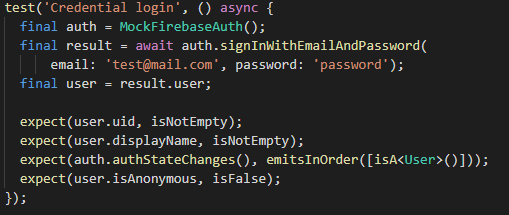
\includegraphics[scale=0.75]{slike/login.PNG}
				\centering
				\caption{Prijava u sustav}
				\label{fig:login}
			\end{figure}
			
			Ispitni slučaj na slici \ref{fig:userFetch} vraća korisnika koji je prijavljen.
			
			\begin{figure}[h]
				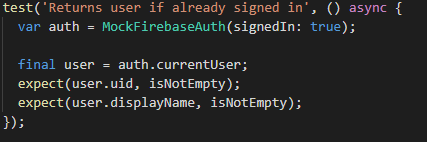
\includegraphics[scale=0.75]{slike/userFetch.PNG}
				\centering
				\caption{Prikaz prijavljenog korisnika}
				\label{fig:userFetch}
			\end{figure}
			
			\eject
			
			
			Kod na slici \ref{fig:signOut} provjerava je li odjava korisnika uspješno provedena.
			
			\begin{figure}[h]
				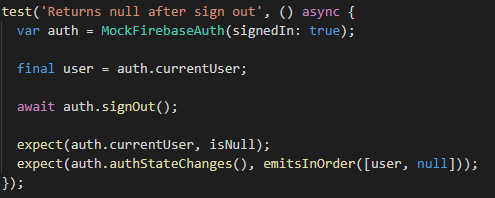
\includegraphics[scale=0.75]{slike/signOut.PNG}
				\centering
				\caption{Provjera odjave}
				\label{fig:signOut}
			\end{figure}
			
			Rezultati testova vidljivi su na slici \ref{fig:unitTests}.
			
			\begin{figure}[h]
				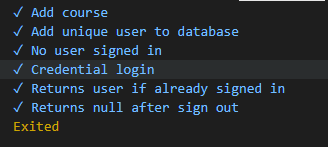
\includegraphics[scale=0.75]{slike/unitTests.PNG}
				\centering
				\caption{Rezultati testova}
				\label{fig:unitTests}
			\end{figure}
			
			Aplikacija je prošla sve testove.
			
			
			\eject
			
			\subsection{Ispitivanje sustava}
			
			Ispitivanje sustava verificira funkcijske i nefunkcijske zahtjeve te prihvatljivost sustava. Automatizirane testove smo proveli pomoću Flutter Drivera.
			
			Ispitni slučaj na slici \ref{fig:wrongCred} simulira pokušaj prijave s neispravnom lozinkom. Nakon unosa e-mail adrese, očekuje se da će se ona nalaziti u svom polju za unos. Jednako tako se očekuje i za lozinku.
			
			\begin{figure}[h]
				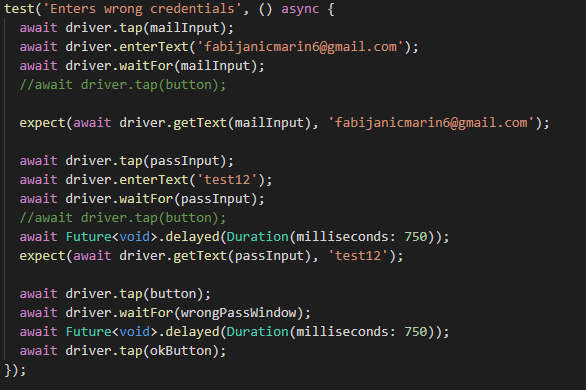
\includegraphics[scale=0.75]{slike/wrongCred.PNG}
				\centering
				\caption{Neispravan unos korisničkih podataka}
				\label{fig:wrongCred}
			\end{figure}
			
			Kod na slici \ref{fig:goodCred} prikazuje prijavu s ispravnom lozinkom. Ovaj put se nakon ponovnog unosa šifre očekuje da će se u polju za unos nalaziti ispravna lozinka, te da će se na pritisak gumba izvršiti prijava.
			
			\begin{figure}[h]
				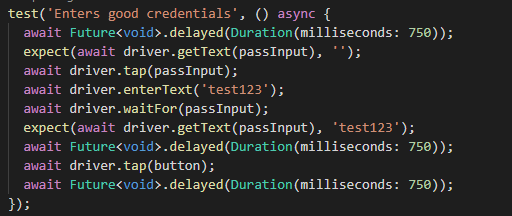
\includegraphics[scale=0.75]{slike/goodCred.PNG}
				\centering
				\caption{Ispravan unos korisničkih podataka}
				\label{fig:goodCred}
			\end{figure}
			
			
			\eject
			
			Kod na slici \ref{fig:wrongName} očekuje da će se, nakon odabira kategorije i težine tečaja, u polju za unos nalaziti naziv tečaja (ovdje je to polje ostavljeno prazno, što se i očekuje). Zatim test očekuje da će se u polju za unos opisa tečaja nalaziti opis, međutim tečaj neće biti dodan jer nije unesen njegov naziv.
			
			\begin{figure}[h]
				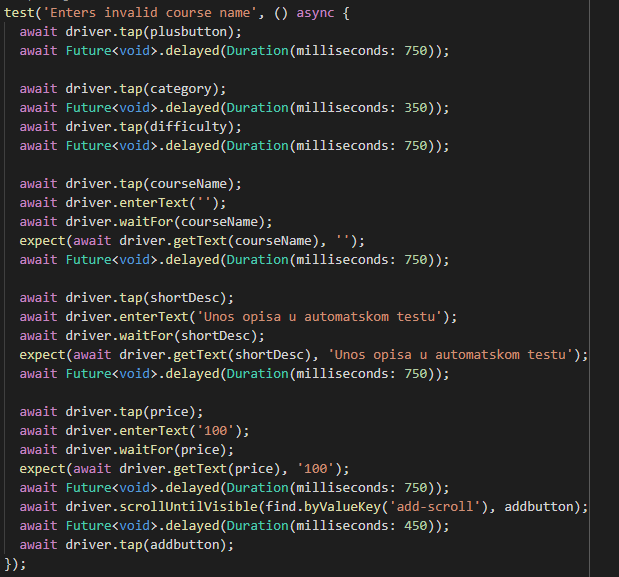
\includegraphics[scale=0.75]{slike/wrongName.PNG}
				\centering
				\caption{Neispravan naziv tečaja}
				\label{fig:wrongName}
			\end{figure}
			
			
			\eject
			
			Kod na slici \ref{fig:validName} očekuje da će se nakon ponovnog unosa naziva tečaja on nalaziti u odgovarajućem polju za unos, te da će se izvršiti dodavanje tečaja.
			
			\begin{figure}[h]
				\includegraphics[scale=0.70]{slike/validName.PNG}
				\centering
				\caption{Unos ispravnog naziva tečaja}
				\label{fig:validName}
			\end{figure}
			
			Slika \ref{fig:editProf} prikazuje kod koji simulira odlazak korisnika na svoj profil i pokušaj izmjene osobnih podataka.
			Korisnik ispravno unosi sve potrebne podatke i uređuje svoj profil. Nakon toga, test se vraća na profilnu stranicu korisnika i provjerava izmijenjene podatke.
			
			\begin{figure}[hbt!]
				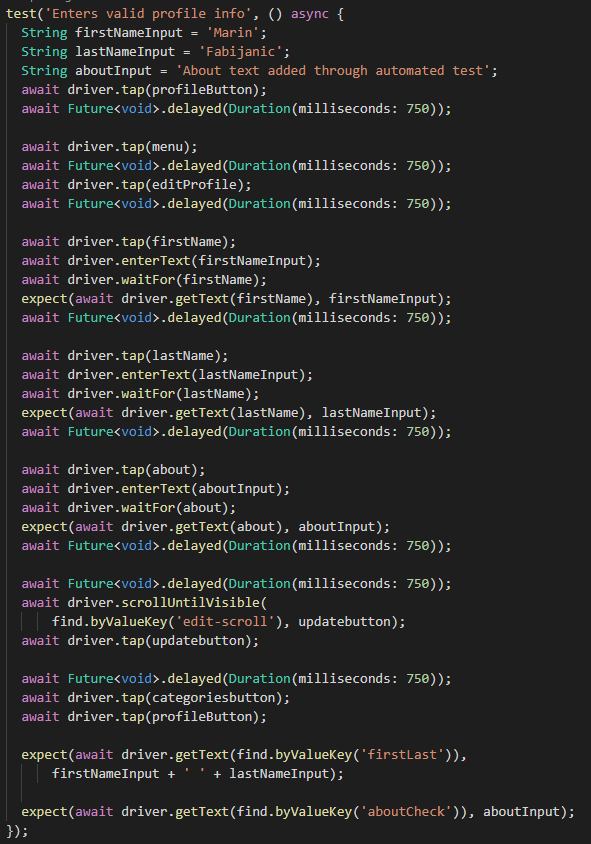
\includegraphics[scale=0.47]{slike/editProf.PNG}
				\centering
				\caption{Uređivanje osobnih podataka}
				\label{fig:editProf}
			\end{figure}
			
			
			\eject
			
			Rezultati testova vidljivi su na slici \ref{fig:integTests}.
			
			\begin{figure}[h]
				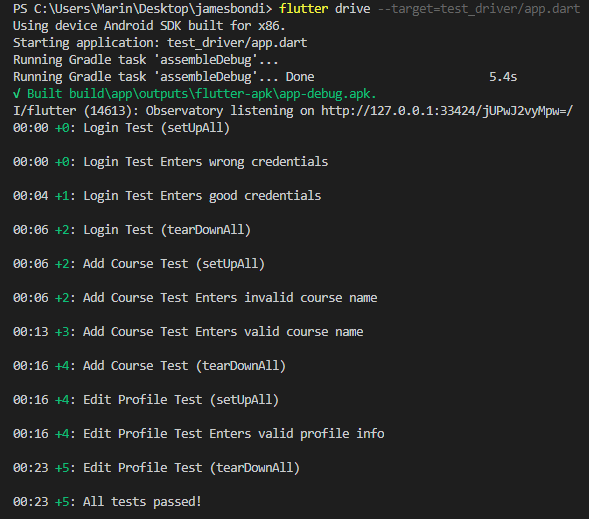
\includegraphics[scale=0.4]{slike/integTests.PNG}
				\centering
				\caption{Rezultati integracijskih testova}
				\label{fig:integTests}
			\end{figure}
			
			Aplikacija je prošla sve testove.
			
			\eject 
		
		
		\section{Dijagram razmještaja}
			
			Dijagram razmještaja opisuje topologiju sustava i usredotočen je na odnos sklopovskih i programskih dijelova. Na slici \ref{fig:Dijagram_razmjestaja} prikazan je specifikacijski dijagram razmještaja koji prikazuje komunikaciju mobilnog uređaja s operacijskim sustavom Android na kojem se nalazi mobilna aplikacija s bazom podataka koja se nalazi u oblaku. Mobilna aplikacija spaja se HTTP protokolom na oblak. U oblaku se unutar Firebase platforme nalazi baza podataka Cloud Firestore, usluga za pohranu podataka Storage i Firebase Authentication za određivanje identiteta korisnika.
			
			
			\begin{figure}[h]
				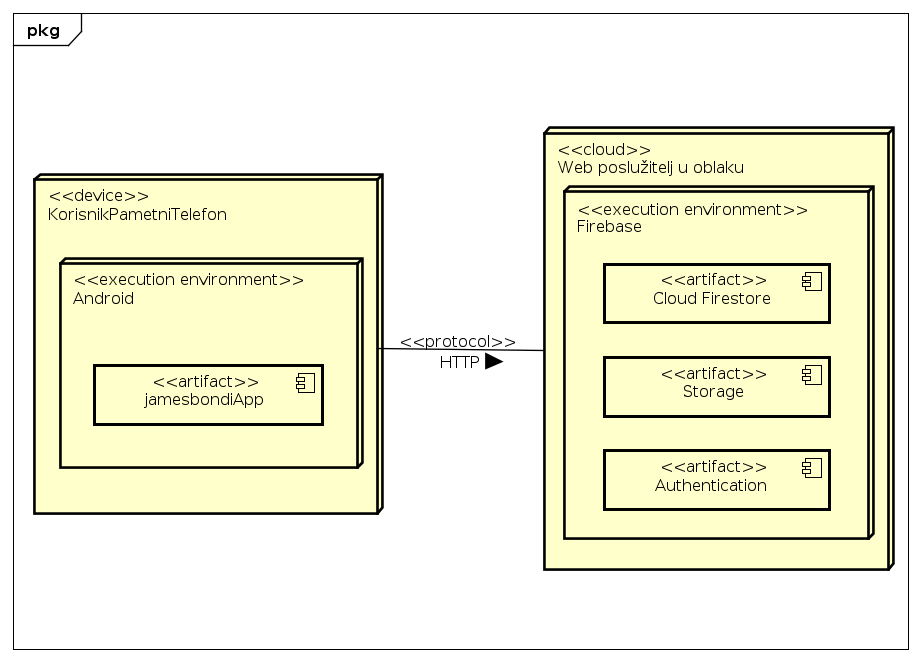
\includegraphics[scale=0.6]{dijagrami/Dijagram_razmjestaja.PNG}
				\centering
				\caption{Dijagram razmještaja}
				\label{fig:Dijagram_razmjestaja}
			\end{figure}
		
			
			\eject 
		
		\section{Upute za puštanje u pogon}
		
			\textbf{\textit{dio 2. revizije}}\\
		
			 \textit{U ovom poglavlju potrebno je dati upute za puštanje u pogon (engl. deployment) ostvarene aplikacije. Na primjer, za web aplikacije, opisati postupak kojim se od izvornog kôda dolazi do potpuno postavljene baze podataka i poslužitelja koji odgovara na upite korisnika. Za mobilnu aplikaciju, postupak kojim se aplikacija izgradi, te postavi na neku od trgovina. Za stolnu (engl. desktop) aplikaciju, postupak kojim se aplikacija instalira na računalo. Ukoliko mobilne i stolne aplikacije komuniciraju s poslužiteljem i/ili bazom podataka, opisati i postupak njihovog postavljanja. Pri izradi uputa preporučuje se \textbf{naglasiti korake instalacije uporabom natuknica} te koristiti što je više moguće \textbf{slike ekrana} (engl. screenshots) kako bi upute bile jasne i jednostavne za slijediti.}
			
			
			 \textit{Dovršenu aplikaciju potrebno je pokrenuti na javno dostupnom poslužitelju. Studentima se preporuča korištenje neke od sljedećih besplatnih usluga: \href{https://aws.amazon.com/}{Amazon AWS}, \href{https://azure.microsoft.com/en-us/}{Microsoft Azure} ili \href{https://www.heroku.com/}{Heroku}. Mobilne aplikacije trebaju biti objavljene na F-Droid, Google Play ili Amazon App trgovini.}
			
			
			\eject 